% !TeX root = main.tex
\input{header.tex}

\subject{V44}
\title{Röntgenreflektometrie}
\date{%
  Durchführung: 30. Mai 2022
  \hspace{3em}
  Abgabe: \today
}

\begin{document}

\maketitle
\thispagestyle{empty}
\tableofcontents
\newpage

\section{Theorie}
\label{sec:Theorie}



\subsection{Ionenkristalle}
Ein Ionenkristall setzt sich zusammen aus Kationen (positiv geladen) und Anionen (negativ geladen),
welche in einer Gitterstruktur angeordnet sind. Im Falle von Kaliumbromid ist dies in einer fcc-Struktur.
In einem perfektem Krtistall wären alle Plätze der Struktur durch diese Ionen alternierend besetzt.
Dies würde einen homogenen, elektrisch neutralen Kristall ergeben.
In reelen Kristallen hingegen befinden sich immer wieder Störstellen,
die die Struktur des Gitters unterbrechen.
Für diesen Versuch besonders interessant sind die Leerstellen,
also leere Gitterplätze.
Diese können ihre Position im Kristall verändern,
indem Ionen ihren Platz einehmen und einen leeren Platz hinterlassen.

Bei der Dotierung werden dem Ionenkristall Fremdatome im geringen Maße hinzugefügt,
welche den Platz einer Leerstelle einehmen können.
Dabei muss auf mikoskopischer Ebene Ladungsneutralität herschen.
Sobald das Fremdatom eine Ladungsänderung im Kristall vornimmt,
lösen sich eine entsprechende Anzahl an Ionen aus ihren Gitterplätzen und füllen Leerstellen
oder wandern an die Oberfläche.
Bei einem durch Strontium dotierten Kaliumbromidkristall
ersetzt ein zweifach positiv geladenes Strontium-Ion ein einfach positiv geladenes Kalium-Ion.
Zum mikroskopischen Ladungsausgleich entsteht in der Umgebeung eine Leerstelle 
und das Kation wandert im Festkörper an den Rand.
Leerstelle und Dotierung bilden hier einen Dipol.



\subsection{Dipole und Dipolrelaxion in Ionenkristallen}
Ein Dipol ist die Anordnung zweier entgegengesetzter Ladungen.
Das zugehörige Dipolmoment $\vec{p}$ berechnet sich durch
\begin{equation*}
    \vec{p} = \sum_i q_i \cdot \vec{r_i}
\end{equation*}
mit den Ladungen $q_i$ an den Orten $\vec{r_i}$ 
und zeigt immer in Richtung der positiven Ladung.
Innerhalb eines elektrischen Feldes richten sich diese Dipole entlang der Feldlinien aus,
um einen Zustand minimaler Energie einnehmen zu können.
Daduch bildet sich eine Vorzugsrichtung für das Dipolmoment.
Ohne elektrisches Feld sind die Dipole so verteilt, 
dass sich ihr Gesammtdipolmoment zu Null addiert.

Die Zeit welche die Dipole nach der Polarisation benötigen,
um eine Richtungsänderung zu vollführen nennt sich Relaxionszeit:
\begin{equation}
    \tau(T) = \tau_0 \cdot \exp\left(\frac{W}{k_B T}\right) , \tau_0 =\tau(\infty).
\end{equation}
Sie ist abhängig von der Aktivierungsenergie $W$,
welche benötigt wird,
um die Coulomb-Barriere des Ionengitters zu überwinden,
so wie der Temperatur $T$.
Zu erkennen ist,
dass die Relaxionszeit bei niedrigen Temperaturen niedrig und bei hohen hoch ist.
Daher wird der Ionenkristall bei etwa \qty{320}{\kelvin} in ein E-Feld gegeben,
damit die Einschaltdauer möglichst groß gegenüber der Relaxationszeit ist und eine Polarisation im Kristall möglich ist.
Durch das anschließende Abkühlen wird diese Polarisation auch bei abgeschaltetem E-Feld quasi festgehalten. 



\subsection{Der Depolarisationsstrom}
Bei der stattfindenden Depolarisation wird ein Strom induziert,
welcher gemessen werden kann. 
Aus diesem Depolarisationsstrom lassen sich die Größen Aktivierungsenergie und Relaxionszeit bestimmen.
Ermittelt werden kann der Depolarisationsstrom durch zwei Ansätze.

\subsubsection{Polarisationsansatz}
Der Depolarisationsstrom beträgt dabei im allgemeinen
\begin{equation}
    i(T) = -\frac{\mathrm{d}P(t)}{\mathrm{d}t}\,.
    \label{eqn:polstrom2}
\end{equation}
Die Polarisationsrate hängt von der übrigen Polarisation zur Zeit $t$
und von der Relaxationsrate $\tau(T)$ ab.
\begin{equation}
    \frac{\text{d}{P(t)}}{\text{d}{t}} = -\frac{P(t)}{\tau(T)}
    \label{eqn:polrate}
\end{equation}
Aus den beiden Gleichungen \eqref{eqn:polrate} und \eqref{eqn:polstrom2} ergibt sich daher
\begin{equation}
    i(T) = \frac{P(t)}{\tau(T)}\,.
    \label{eqn:i_t_polstart}
\end{equation}
Gleichung \eqref{eqn:polrate} integriert führt zu einen Zusammenhang für $P(t)$
\begin{equation}
    P(t) = P_{0} \exp\!\left(-\frac{t}{\tau(T)}\right)\,,
\end{equation}
welcher sich mit Gleichung \eqref{eqn:i_t_polstart} zu
\begin{equation}
    i(T) = \frac{P_0}{\tau} \exp\!\left(-\frac{t}{\tau(T)}\right) 
\end{equation}
ergibt.
Die Zeit $t$ wird nun als Integral über den Startpunkt bis zum Beginn des Depolarisationsstroms beschrieben
\begin{equation}
    i(T) = \frac{P_{0}}{\tau} \exp\!\left(-\int_0^t \frac{\text{d}{t}}{\tau(T)}\right)\,.
\end{equation}
Bei einer konstanten Heizrate $b$ nimmt der der Depolarisationsstrom die Form
\begin{equation}
    i(T) = \frac{P_0}{\tau} \exp\!\left(-\int_{T_0}^T
      \exp\!\left(- \frac{W}{k_B T}\right) \text{d}{T}\right)
    \label{eq:final}
\end{equation}
an.

Zur Berechnung der Aktivierungsenergie $W$ und der Relaxationszeit wird angenommen,
dass $W$ groß im Vergleich zur thermischen Energie $k_B T$
und die Temperaturdiferenz $T - T_0$ gering ist.
Mit der Annahme wird aus \refeq{eq:final}
\begin{equation}
    i(T) = \frac{P_0}{\tau} \exp\!\left(-\int_{T_0}^T
      \exp\!\left(- \frac{W}{k_B T}\right) \text{d}{T}\right) \approx 0
\end{equation}
und der Ausdruck für den Strom vereinfacht sich zu 
\begin{equation}
    I(T) \approx \frac{p^2E}{3k_B T_0}\cdot\frac{N_0}{\tau_0}\cdot\exp{\frac{-W}{k_B T}}.
\end{equation}
Mit dem Bilden des Logarithmus ergibt sich
\begin{equation}
    \log(I(T)) = \text{const} -\frac{W}{k_B T}
    \label{eq:W1}
\end{equation}
was in der Auswertung für eine lineare Ausgleichsrechnung zwischen $\log(I)$
und $T^{-1}$ zur Bestimmung von W verwendet wird.
Für die Relaxationszeit gilt am Maximum 
\begin{equation}
    \tau_{\text{max}} (T_{\text{max}}) = \frac{k_\text{B} T^2_{\text{max}}}{b W}\, ,
\end{equation}
woraus die charakteristische Relaxationszeit $\tau_0$ 
\begin{equation}
    \tau_0 = \tau_{\text{max}} (T_{\text{max}}) \exp \left(- \frac{W}{k_{\text{B}} \cdot T_\text{max}}\right) = \frac{k_\text{B} T^2_{\text{max}}}{b W} \cdot\exp \left(- \frac{W}{k_{\text{B}} \cdot T_\text{max}}\right)
    \label{eq:relax}
\end{equation}
berechnet werden kann.


\subsubsection{Stromdichtenansatz}
Der zweite Ansatz zur Bestimmung der Aktivierungsenergie $W$ geht über die Annahme,
dass die Änderung der Polarisation $P$ mit der Zeit zum Betrag der Stromdichte $j(T)$
entspricht.
Die Änderung der Polarisation $P$ ist definiert als
\begin{equation*}
    \frac{\text{d}P}{\text{d}t} = -\frac{P(t)}{\tau(T)}\, .
\end{equation*}
Nach umstellen und erweitern mit $\frac{\text{d}T}{\text{d}T}$ folgt 
\begin{equation*}
    \tau(T) = P(T) \cdot \frac{\text{d}T}{\frac{\text{d}P}{\text{d}t}\text{d}T } =  \frac{P(t)}{b} \frac{\text{d}T}{\text{d}P}\,.
\end{equation*}
Durch erneute Erweiterung mit $\frac{\text{d}t}{\text{d}t}$ ergibt sich:
\begin{equation*}
    \tau(T) = \frac{P(t)}{b} \frac{\frac{\text{d}T}{\text{d}t}}{\frac{\text{d}P}{\text{d}t}}
\end{equation*}
Nun wird durch die vorhergehende Annahme und $P =\int\text{d}P$ der Term für die Relaxationszeit umgeformt zu: 
\begin{equation*}
    \tau(T) = \frac{\int \frac{\text{d}P}{\text{d}t} \text{d}T}{I(T) \cdot b} = \frac{\int_T^\infty I(T') \, \text{d}T'}{I(T) \cdot b}
\end{equation*}
Einsetzen und die Gleichung zur Aktivierungsenergie $W$ umstellen ergibt:
\begin{equation}
    W = k_\text{B} T \cdot \ln\left( \frac{\int_T^\infty I(T') \, \text{d}T'}{b \tau_0 \cdot I(T)}\right)
    \label{eq:Int}
\end{equation}
Somit lässt sich nun die Aktivierungsenergie $W$ berechnen. In der Praxis wird die obere Integrationsgrenze von $\infty$ in $T^*$ geändert, mit
$I\left(T^*\right)\approx 0$. Demnach soll $T^*$ groß genug sein, um eine Gleichverteilung der Dipole hervorzurufen. 
\section{Durchführung}
\label{sec:Durchführung}
Der Versuch wurde an einem D8-Labordiffraktometer durchgeführt.
Eine Röntgenröhre, die mit \qty{40}{\kilo\volt} und \qty{35}{\milli\ampere} in Betrieb ist,
bestrahlt eine Probe. Ein Detektor erfasst dabei die reflektierte Strahlung.
Die Probe, ein mit Polymerfilm beschichteter Siliziumwafer, muss durch eine Vielzahl von Scans zunächst justiert werden

\subsection{Justierung}
\subsubsection*{Detektorscan}
Unanbhängig von der Probe werden Röhre und Detektor auf eine Ebene gebracht. Nun fährt der Detektor einen kleinen Winkelbereich um den Strahl der Röhre ab.
Das Maximum der aufgenommenen Intensität, die einer Gaußglocke ähnelt, ist fortan der neue Nullpunkt der Detektorausrichtung.

\subsubsection*{Z-Scan}
Der Z-Scan dient zur Höhenausrichtung der Probe.
Dabei wird die Probe leicht in der Höhe verschoben.
Richtig justiert ist sie,
wenn sie parallel zum Strahl steht (siehe Detektorscan) und die halbe Intensität des Primärstrahls abschattet.
Die Intensität des Strahls nimmt desto mehr ab, je weiter sich die Probe im Strahl befindet.
Die Probe wird soweit in den Strahl gefahren, bis eine halbe Abschattung zu erkennen ist. 

\subsubsection*{Rockingscan}
Dennoch besteht die Möglichkeit, dass die Probe nicht parallel zur Ausbreitungsrichtung des Röntgenstrahls steht.
Demnach wird die Probe ungleichmäßig getroffen. Um auch diese Hürde zu bewältigen drehen sich beim Rockingscan
Röhre und Detektor mit konstanter Winkelsumme um die Probe um diese im Drehpunkt des Diffraktometers zu zentrieren.

\subsubsection*{Feinjustierung}
Nach den ersten drei Scans folgt ein weiter Z-Scan um nach der Drehung wieder die Hälfte abzudecken.
Anschließend wird noch einmal der Rockingscan mit einem abschließendem Z-Scan wiederholt um endgültig mit der Messung anzufangen.

\subsection{Messung}
Gemessen werden ein Reflektivitätsscan und ein diffuser Scan.
Hierzu wird das eingerichtete Programm, XRD Commander, gemäß der Anleitung\cite{sample} genutzt.

Beim Reflektivitätsscan sind der Röhren- und Detektorwinkel gleich groß. Es wird in
einem Bereich von 0° bis 2,5° mit einer Schrittweite von 0,005° und einer Messzeit von
\qty{5}{\second} gemessen.
Bei dem diffusen Scan ist der Detektorwinkel um 0,1° gegenüber dem Röhrenwinkel
verschoben. Jedoch bleibt der Vorgang der gleiche. Durch diesen Scan, kann später die wahre Reflektivität berechnet werden.
\section{Auswertung}
\label{sec:Auswertung}
\subsection{Messung der Molwärme}

Die Molwärme $C_V$ bei konstantem Volumen experimentell zu bestimmen,
gestaltet sich aufgrund der dadurch auftretenden hohen Drücke schwierig.
Daher wird zuerst $C_p$ bei konstantem Druck bestimmt 
und anschließend wird durch den Zusammenhang in Gleichung \refeq{eq:korrekt} $C_V$ bestimmt.
Mit der zugeführten Energeie
\begin{equation*}
    E = U\cdot I \cdot \Delta t,
\end{equation*}
lässt sich die Volumenabhängige Molwärme $C_p$ bestimmen
\begin{equation*}
    C_p = \frac{M}{m} \cdot \frac{E}{\Delta T}.
\end{equation*}
Dabei bezeichnet $U$ die gemessene Spannung,
$I$ die Stromstärke, 
$\Delta t$ das Zeitintervall zwischen zwei Messungen,
$\Delta T$ den temperaturunterschied,
$M$ die molare Masse der Probe und
$m$ die Probenmasse.
Die  Werte sind in Tabelle \eqref{tab:Messwerte} dargestelt.
\begin{table}[ht]
    \centering
    \caption{Die aufgenommene Wärmemenge und $C_V$ berechnet mit den Messwerten für Strom,Spannung, Zeit und Temperatur.}
    \begin{tabular}{rrrrrr}
    \toprule
    U/V & I/mA & $\Delta t$/s & $\Delta T$ K & E/J & $C_p$  \\ 
    \midrule
    16   & 150  & 0   & 0   & 0   & 0    \\
    15.85& 151.3& 321 & 10.1& 771 & 14.1 \\
    15.99& 152.3& 353 & 10.2& 848 & 15.5 \\
    16.07& 152.9& 406 & 10  & 989 & 18.3 \\
    16.13& 153.3& 388 & 10  & 953 & 17.6 \\
    16.17& 153.5& 410 & 9.8 & 1014& 19.0 \\
    16.21& 153.8& 459 & 10.1& 1050& 20.9 \\ 
    16.24& 153.9& 421 & 9.7 & 1108& 20.0 \\
    16.26& 154.1& 443 & 10  & 1181& 20.5 \\
    16.28& 154.2& 471 & 10  & 1186& 21.8 \\
    16.29& 154.3& 472 & 9.8 & 1382& 22.4 \\
    16.30& 154.4& 550 & 10.1& 1047& 25.3 \\
    16.31& 154.5& 416 & 9.9 & 1094& 19.6 \\
    16.32& 154.5& 434 & 9.9 & 1346& 20.3 \\
    16.32& 154.5& 534 & 10  & 1055& 25   \\
    16.32& 154.6& 418 & 10  & 1027& 19.5 \\
    16.32& 154.7& 407 & 9.8 & 1243& 19.4 \\
    16.32& 154.6& 492 & 9.8 & 2687& 23.3 \\
    16.32& 154.7& 1065& 9.9 & 199 & 50.2 \\
    16.32& 154.6& 79  & 10.2& 1071& 3.6  \\
    16.31& 154.7& 424 & 10.2& 1309& 19.4 \\
    16.31& 154.7& 519 & 9.8 & 358 & 24.8 \\
    16.31& 154.8& 142 & 10.1& 1123& 6.5  \\
    \bottomrule
    \end{tabular}
    \label{tab:Messwerte}
\end{table}

Mit dem Linearen Ausdehnungskoeffizienten $\alpha$ aus \cite*{sample} wird $C_V$ berechnet.
Die Werte für den Temperaturabhängigen Ausdehnungskoeffizienten sind mit Ausgleichsgerade in Abbildung \refeq{fig:alpha} dargestellt.
\begin{figure}[h] 
  \centering
     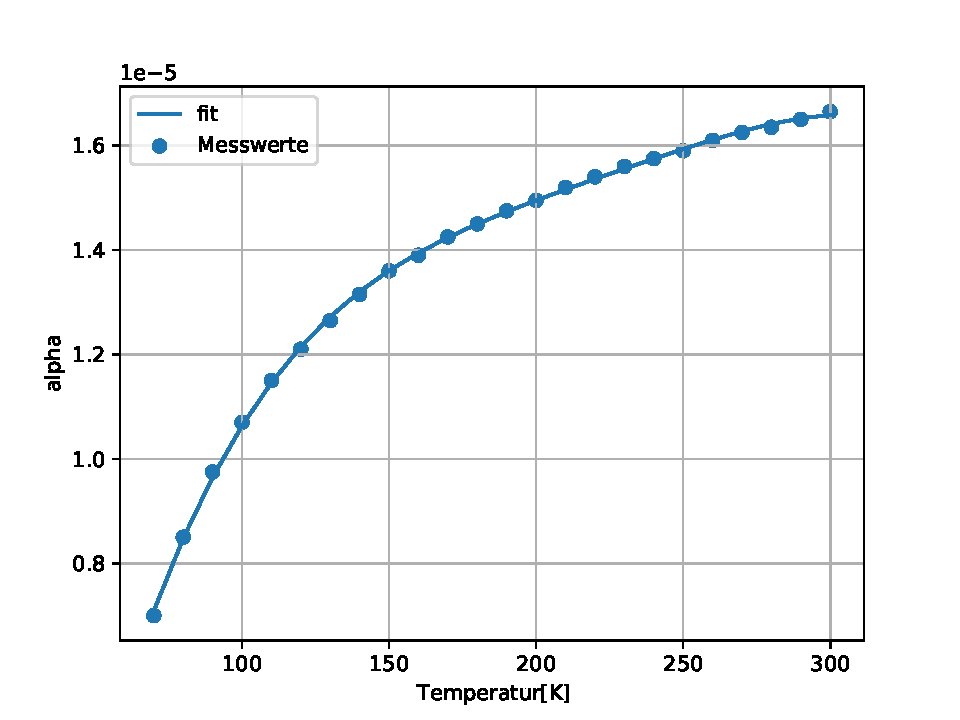
\includegraphics[width=0.7\textwidth]{Auswertung/Plots/alpha.pdf}
  \caption{Fit für den linearen Ausdehnungskoeffizienten}
  \label{fig:alpha}
\end{figure}
Daraus ergibt sich mit der Korrekturformel \refeq{eq:korrekt}, die in Abbildung \ref{fig:C_v} dargestelte Temperaturabhängigkeit der Molwärme.
\begin{figure}[h] 
    \centering
       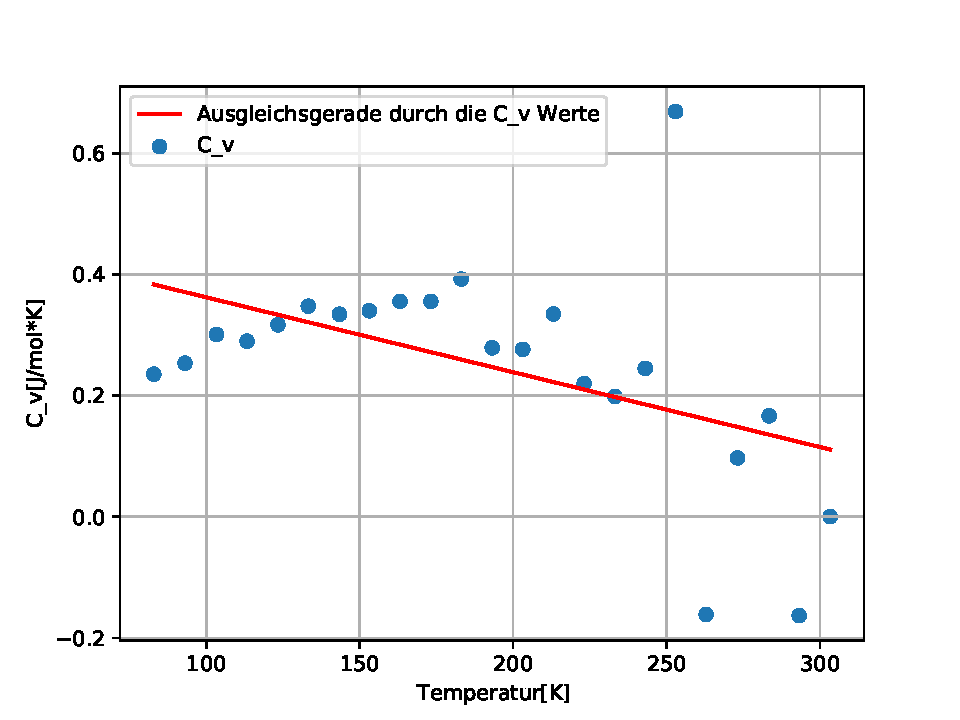
\includegraphics[width=0.7\textwidth]{Auswertung/Plots/C_v.pdf}
    \caption{Die Molwärme in Abhängigkeit von der Temperatur}
    \label{fig:C_v}
\end{figure}



\subsection{Bestimmung der Debye-Temperatur}
Um die Debey-Temperatur $\theta_D$ zu bestimmen wird die Tabelle \ref{tab:debey} verwendet werden.
\begin{figure}[h] 
    \centering
       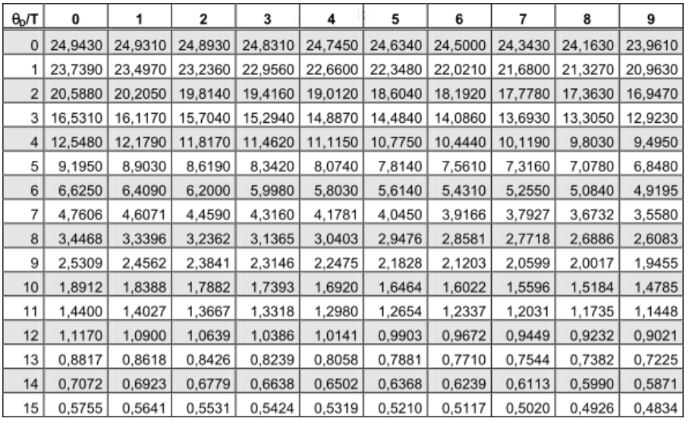
\includegraphics[width=0.8\textwidth]{Tabellen/debey.JPG}
    \caption{Werte der Debye-Funktion.}
    \label{tab:debey}
\end{figure}
Diese sind in Tabelle \ref{tab:debey2} dargestellt.
\begin{table}[ht]
    \centering
    \caption{Die aufgenommene Wärmemenge und $C_V$ berechnet mit den Messwerten für Strom, Spannung, Zeit und Temperatur.}
    \begin{tabular}{rrrr}
    \toprule
    T/K & $C_V$ & $\frac{\theta_D}{T}$ & $\theta_D$  \\ 
    \midrule
    82.9 & 14.1& 3.6& 298.4 \\ 
    93   & 15.4& 3.3& 306.9 \\
    103.3& 18.3& 2.6& 268.5 \\
    113.3& 17.6& 2.7& 305.9 \\
    123.4& 19  & 2.4& 296.1 \\
    133.2& 20.8& 1.9& 253   \\
    143.4& 20.0& 2.1& 301.1 \\
    153.1& 20.5& 2.0& 306.2 \\
    163.1& 21.8& 1.7& 277.2 \\
    173.2& 22.3& 1.5& 259.8 \\
    183.0& 25.3& 0  & 0     \\ 
    193.2& 19.5& 2.3& 444.3 \\
    203.1& 20.3& 2.1& 426.5 \\
    213.1& 24.9& 0  & 0     \\ 
    223.1& 19.3& 2.3& 513.1 \\
    233.2& 19.2& 2.4& 559.6 \\
    243  & 23.2& 1.2& 291.6 \\
    252.9& 50  & 0  & 0     \\ 
    262.9& 3.4 & 8.0& 2103.2 \\
    173.1& 19.1& 2.4& 415.44 \\
    283.4& 24.6& 0.5& 151.7 \\
    293.2& 6.32& 6.2& 1817.84 \\
    \bottomrule
    \end{tabular}
    \label{tab:debey2}
\end{table}
Es ergibt sich ein Mittelwert von
\begin{equation*}
    \frac{\theta_D}{T}\cdot T =  443.08 K
\end{equation*}

Aus der Forderung 
\begin{equation}
    \int_0^{\omega_\text D} Z(\omega) d\omega = 3 N_\text L
\end{equation}
kann die Debye-Temperatur für ein gegebenes Material auch bestimmt werden. Dazu wird das Integral über die Verteilungsfunktion 
\begin{equation}
    Z(\omega)d\omega = \frac{L^3}{2\pi^2}\omega^2\left(\frac{1}{v_\text{l}^3}+\frac{2}{v_{\text{t}}^3}\right)d\omega.
\end{equation}
ausgeführt:
\begin{align*}
	\int_0^{\omega_D} \frac{L^3}{2\pi^2}\omega^2\left(\frac{1}{v_\text{l}^3}+\frac{2}{v_\text{tr}^3}\right) d\omega &\overset{!}{=} 3 N_L\\
	\frac{L^3}{6\pi^2}\omega_D^3\left(\frac{1}{v_\text{l}^3}+\frac{2}{v_\text{tr}^3}\right)  &= 3N_L\\
	\left[\frac{18\pi^2N_L}{L^3}\left(\frac{1}{v_\text{l}^3}+\frac{2}{v_\text{tr}^3}\right)^{-1} \right]^{\frac{1}{3}} &= \omega_D \,\text.
\end{align*}
Die Größe $L$ ist die Länge der Probe, welche nicht gegeben ist. Diese kann aber mittels einer Umrechnung der Loschmidtschen Zahl $N_L$ eliminiert werden. Es ergibt sich:
\begin{align*}
	L^3 = V &= \frac{m}{\rho_\text{Cu}}\qquad N_L = N_A\frac{m}{M}\\
	\Rightarrow \frac{N_L}{L^3} &= N_A\frac{\rho_\text{Cu}}{M}\,\text.
\end{align*}
Dabei ist $N_A$ die Avogadrokonstante.
Mit den Werten $m = \SI{342}{\gram}$, $v_\text{l} = \SI{4.7}{\kilo\metre\per\second}$ und $v_\text{tr} = \SI{2.26}{\kilo\meter\per\second}$ kann über
\begin{equation*}
	\theta_D = \frac{\hbar\omega_D}{k_\text{B}}= \frac{\hbar}{k_\text{B}}\left[\frac{18\pi^2\rho_\text{Cu} N_A}{M}\left(\frac{1}{v_\text{l}^3}+\frac{2}{v_\text{tr}^3}\right)^{-1} \right]^{\frac{1}{3}} = \SI{331.991}{\kelvin}
\end{equation*} bestimmt werden. Dabei sind $k_B$ die Boltzmannkonstante und $\hbar$ das reduzierte Plancksche Wirkungsquantum.


\section{Diskussion}
\label{sec:Diskussion}

Der bei der Justierung des Strahls gemessene Geometriewinkel $\alpha = 0.4^°$ weicht leicht vom Literaturwert $\alpha_{t} = 0,687^°$ ab.
Somit war die Justierung erfolgreich, wenn auch nicht optimal.
Auch die über die Kiessig-Oszillation berechnete Schichtdicke weicht nur geringfügig zwischen dem gemessenen 
und den durch Parrat berechneten Werten ab.
\begin{align*}
    d_{Kiessig} &= 882,4 \text{ \AA} \\
    d_{Parrat} &= 860 \text{ \AA}
\end{align*}
Dies folgt wohl der Verbesserungsmöglichkeit der Justierung.
Ebenso ist die zerkratzte Wafer-Oberfläche nicht zu vernachlässigen.
Gerade beim Einstellen der Rauigkeitsparameter des Parrat Algorithmus spielt sie eine entscheidene Rolle.
Dies lässt sich auch an den Dispersionswerten erkennen.
\begin{align*}
    \delta_{Poly} &= 0.3 \cdot 10^{-6} m\\
    \delta_{Si} &= 6.3 \cdot 10^{-6} m 
\end{align*}
Die Literaturwerte \cite{wert} liegen bei:
\begin{align*}
    \delta_{Poly} &= 3.5 \cdot 10^{-6} m\\
    \delta_{Si} &= 7.6 \cdot 10^{-6} m
\end{align*}
Während die Abweichung von Silizium bei $\qty{20}{\percent}$ liegt, beträgt die von Polystrol fas $\qty{1000}{\percent}$,
was auf einen systematischen Fehler hinweißt.
Diese hohe Unsicherheit bei der Dispersion von Polystrol erkennt man auch im Vergleich der kritischen Winkel.
\begin{align*}
    \alpha_{Poly} &= 0,068^°  \\
    \alpha_{Si} &= 0,214^°
\end{align*}
Die Literaturwerte \cite{wert} liegen bei:
\begin{align*}
    \alpha_{Poly} &= 0,153^°  \\
    \alpha_{Si} &= 0,223^°
\end{align*}
Insgesamt liegt eine gewisse Fehleranfälligkeit auf das Einstellen der Parratt-Parameter per Hand.
Viel erheblicher fällt die nicht oütimal glatte Oberfläche der Probe ins Gewicht,
welche durch ihre hohe Rauigkeit für Messfehler sorgt. 
Die Parrat-Kurve beschreibt die gemessene Reflektivität aber genau genug, 
so dass dem Ergebnis eine Aussagekraft zugeschrieben werden kann.
\newpage
\section{Anhang}

\begin{python}
    import numpy as np
    import matplotlib.pyplot as plt

    def parratt(a_i, delta_1, delta_2, sigma_1, sigma_2, d_2, b_1, b_2):
        n_2 = 1.0 - delta_1 +b_1
        n_3 = 1.0 - delta_2 + b_2
        a_i = np.deg2rad(a_i)
        k = 2 * np.pi / wl
        kd_1 = k * np.sqrt(n_1 ** 2 - np.cos(a_i, dtype = np.complex) ** 2)
        kd_2 = k * np.sqrt(n_2 ** 2 - np.cos(a_i, dtype = np.complex) ** 2)
        kd_3 = k * np.sqrt(n_3 ** 2 - np.cos(a_i, dtype = np.complex) ** 2)
     
        
        r_12 = (kd_1 - kd_2) / (kd_1 + kd_2) * np.exp(-2 * kd_1 * kd_2 * sigma_1 ** 2)
        r_23 = (kd_2 - kd_3) / (kd_2 + kd_3) * np.exp(-2 * kd_2 * kd_3 * sigma_2 ** 2)

        x_2 = np.exp(-2j * kd_2 * d_2) * r_23
        x_1 = (r_12 + x_2) / (1 + r_12 * x_2)

        return np.abs(x_1) **2

    #Import Messwerte
    ref_x, ref_y = np.genfromtxt('Messwerte/omega_tet.txt', unpack=True)
    diff_x, diff_y = np.genfromtxt('Messwerte/diffusor.txt' , unpack=True)

    #Reflektivität
    I_0 = 1114508.0792544584
    R_ref = ref_y / (5 * I_0)
    R_diff = diff_y / (5 * I_0)
    R= R_ref - R_diff

    #Parratt Parameter
    n_1 = 1.0               #Brechungsindex Luft
    d_1 = 0.0               #Schichtdicke Luft
    d_2 = 8.6 * 10 ** (-8) #Schichtdicke der Porbe
    wl = 1.54e-10           #Wellenlänge

    delta_1 = 0.3 * 10 ** (-6)
    delta_2 = 6.3 * 10 ** (-6)
    sigma_1 = 1.0 * 10 ** (-10) 
    sigma_2 = 5.5 *10 ** (-10)
    b_1 = (delta_1 / 200) * 1j   # Aus L. G. Parratt. „Surface Studies of Solids by Total Reflection of X-Rays“.
    b_2 = (delta_2/ 40) * 1j


    print(delta_1, delta_2, sigma_1, sigma_2, d_2, b_1, b_2)
    par = parratt(ref_x, delta_1, delta_2, sigma_1, sigma_2, d_2, b_1, b_2)


    #Kritischer Winkel
    a_Poly = np.rad2deg(np.sqrt(2 * delta_1))
    a_Si = np.rad2deg(np.sqrt(2 * delta_2))
    print('Kritischer Winkel Polys:', a_Poly)
    print('Kritischer Winkel Silicium: ', a_Si)

    #Plot
    plt.plot(ref_x, R, '-', label = 'Reflektivität mit Geometriefaktor')
    plt.plot(ref_x, par, '-', label = 'Parratt-Kurve')
    plt.xlabel('\u03B1 / °')
    plt.ylabel('R')
    plt.yscale('log')
    plt.grid()
    plt.legend()
    plt.savefig('Graphen/Parrat_Algorthmus.pdf')
\end{python}



\nocite{numpy}
\nocite{matplotlib}
\nocite{scipy}
\nocite{cheat}
\newpage
\printbibliography{}


\end{document}
